\documentclass[tikz,border=10pt, margin=1cm]{standalone}

% \usepackage[centering,noheadfoot,margin=0.7in]{geometry}
\usepackage[dutch]{babel}
\usepackage{charter}  
\usepackage{booktabs}
\usepackage{array}
\usepackage{multirow}
\usepackage{float}
\usepackage{bm}
\usepackage{tikz}
\usetikzlibrary{shapes.geometric, arrows.meta, positioning}
\setlength{\parindent}{0cm} 

\tikzstyle{startstop} = [rectangle, rounded corners, minimum width=3cm, minimum height=1cm, rounded corners, text centered, draw=black, fill=blue!20]
\tikzstyle{decision} = [rectangle, minimum width=3cm, minimum height=1cm, rounded corners,text centered, draw=black, fill=orange!30]
\tikzstyle{process} = [rectangle, minimum width=3.5cm, minimum height=1cm, rounded corners, text centered, draw=black, fill=green!20]
\tikzstyle{arrow} = [thick,->,>=stealth]

% Laad stijlen via relatieve paden
\newcommand{\path}{C:/Users/danny/Documents/GitHub/Statistiek}
\usepackage{\path/LaTeX/styles/config}
\usepackage{\path/LaTeX/styles/statistics-macros}
\graphicspath{{\path/LaTeX/figures/}}

\usepackage{amsmath, amsfonts, amssymb, amsthm}

\begin{document}
    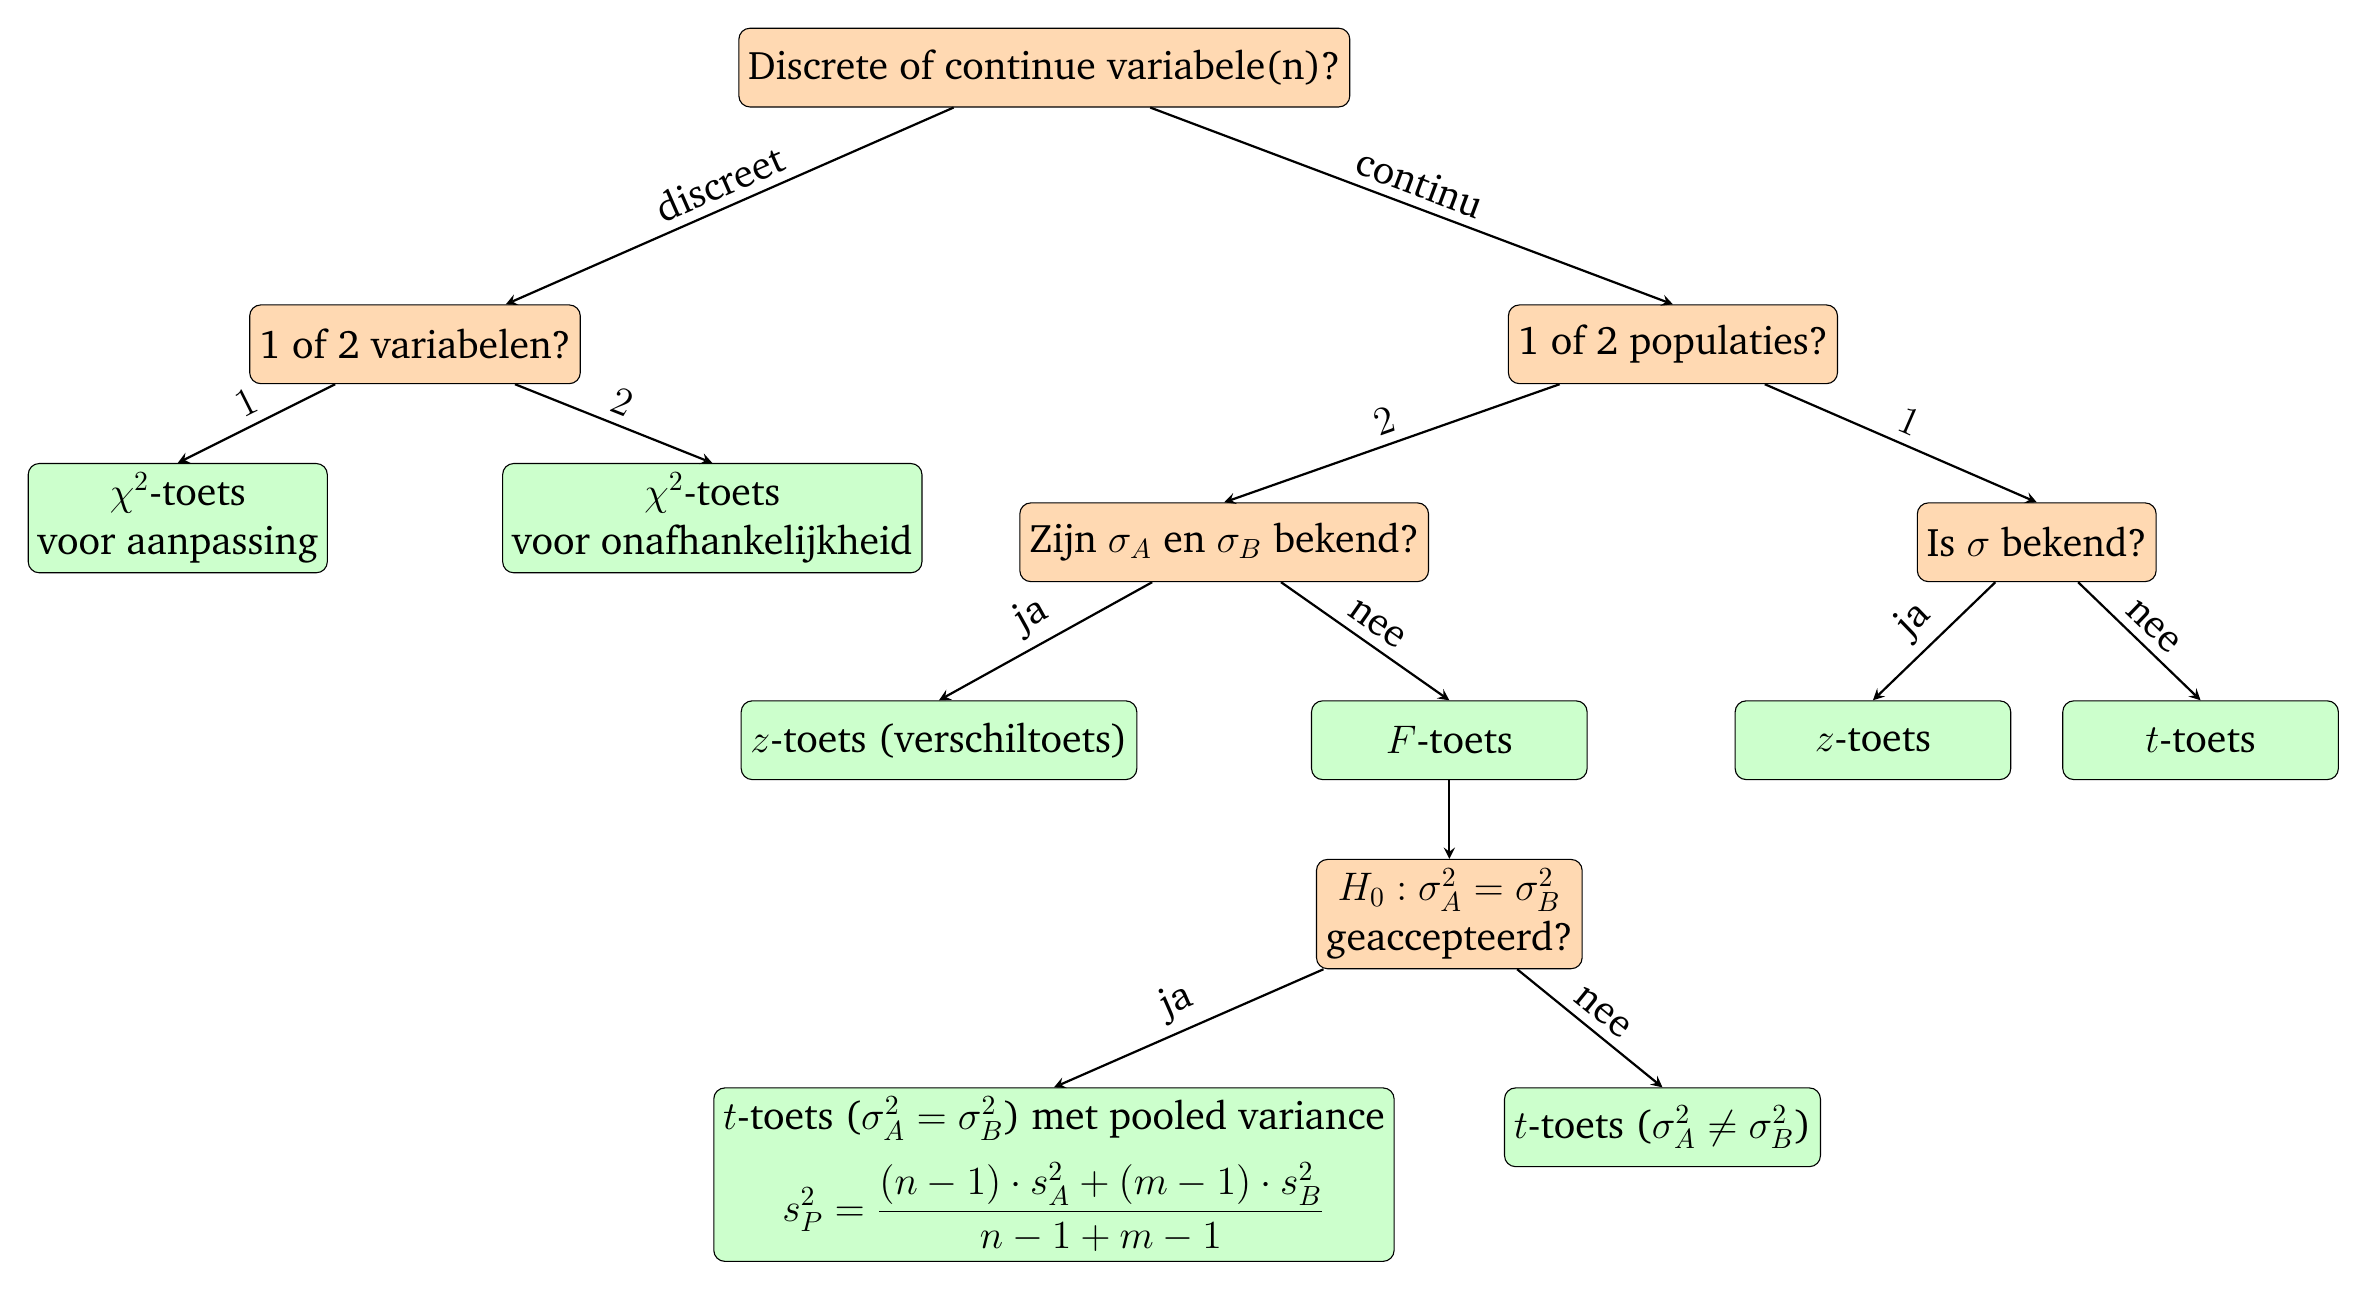
\begin{tikzpicture}[font=\Large, node distance=2cm]

        % Nodes
        \node[decision] (discreteOrContinuous) {Discrete of continue variabele(n)?};

        % Discrete tak
        \node[decision, below left=25mm and 20mm of discreteOrContinuous] (vars) {1 of 2 variabelen?};

        \node[process, below left=10mm and -10mm of vars, align=center] (aanpassing) {$\chi^2$-toets \\ voor aanpassing};
        \node[process, below right=10mm and -10mm of vars, align=center] (onafhankelijkheid) {$\chi^2$-toets \\ voor onafhankelijkheid};
        % Arrows discrete tak
        \draw [arrow] (discreteOrContinuous) -- node[above, sloped] {discreet} (vars);
        \draw [arrow] (vars) -- node[above, sloped] {$1$} (aanpassing.north);
        \draw [arrow] (vars) -- node[above, sloped] {$2$} (onafhankelijkheid.north);

        % Continue tak
        \node[decision, below right=25mm and 20mm of discreteOrContinuous] (populaties) {1 of 2 populaties?};

        \node[decision, below left=15mm and 10mm of populaties] (sigmas) {Zijn $\sigma_A$ en $\sigma_B$ bekend?};
        \node[decision, below right=15mm and 10mm of populaties] (sigma) {Is $\sigma$ bekend?};

        \node[process, below left=15mm and -15mm of sigmas, align=center] (ztoets2) {$z$-toets (verschiltoets)};
        \node[process, below right=15mm and -15mm of sigmas, align=center] (ftoets) {$F$-toets};
        \node[process, below left=15mm and -12mm of sigma] (ztoets) {$z$-toets};
        \node[process, below right=15mm and -12mm of sigma] (ttoets) {$t$-toets};
        
        \node[decision, below=of ftoets, yshift=1cm, align=center] (varEqual) {$H_0: \sigma_A^2 = \sigma_B^2$ \\ geaccepteerd?};

        \node[process, below left=15mm and -10mm of varEqual, align=center] (ttoets2_pooled) {$t$-toets ($\sigma_A^2 = \sigma_B^2$) met \enquote{pooled variance} \\[1ex] $\displaystyle s_P^2 = \frac{(n-1)\cdot s_A^2 + (m-1) \cdot s_B^2}{n-1+m-1}$};
        \node[process, below right=15mm and -10mm of varEqual] (ttoets2) {$t$-toets ($\sigma_A^2 \neq \sigma_B^2$)};

        % Arrows continue tak
        \draw[arrow] (discreteOrContinuous) -- node[above, sloped] {continu} (populaties.north);
        \draw[arrow] (populaties) -- node[above, sloped] {$1$} (sigma.north);
        \draw[arrow] (populaties) -- node[above, sloped] {$2$} (sigmas.north);
        \draw[arrow] (sigma) -- node[above, sloped] {ja} (ztoets.north);
        \draw[arrow] (sigma) -- node[above, sloped] {nee} (ttoets.north);


        \draw [arrow] (sigmas) -- node[above, sloped] {nee} (ftoets.north);
        \draw [arrow] (sigmas) -- node[above, sloped] {ja} (ztoets2.north);
        \draw [arrow] (ftoets) -- node[above, sloped] {} (varEqual.north);
        \draw [arrow] (varEqual) -- node[above, sloped] {ja} (ttoets2_pooled.north);
        \draw [arrow] (varEqual) -- node[above,sloped] {nee} (ttoets2.north);

    \end{tikzpicture}
\end{document}